\section{Methodology}

\subsection{Problem Definition}
The market-making problem addressed in this work involves designing an optimal trading policy for an agent using reinforcement learning (RL). The agent aims to maximize profit while managing risks, particularly inventory risk. The market dynamics are modeled by the limit order book (LOB) and its dynamics, which define how the book evolves over time based on order flow and price movements. Our agent interacts with this environment by quoting bid and ask prices and adjusting offered quantities. As discussed previously, the main challenge for choosing an adequate agent and its policy lies in balancing profitability with risk management, especially regarding inventory at the close of the market, where overnight positions can expose the agent to significant risks.

\subsection{Formal Description of the RL Environment} In modeling the RL environment, we initially utilize a continuous-time Markov chain framework, and later transition to a discrete framework to address computational space constraints. A state space is chosen that best incorporates the historical events of the limit order book into a single observable state, containing both intrinsic and extrinsic features to the agent, as proposed by <multiple references>. Given our performed bibliographical research, we chose the agent's current inventory for the intrinsic feature and a set of indicators for the extrinsic features: the Relative Strength Index (RSI); order imbalance (O); and micro price (MP). Additionally, for a fixed number $D$ of LOB price levels the pair $(\delta^d, Q^d)$, where $\delta^d$ is the half-spread distance for the level $d \leq D$, and $Q^d$ the amount of orders posted at that level is added to the state as a set of tuples, for both the ask and bid sides of the book. The state space can therefore be formally expressed as:
$$
X_t = (I_t, \, RSI_t, \, O_t, \, \text{MP}_t, \, \{ (\delta_t^{d, \text{ask}}, Q_t^{d, \text{ask}}) \}_{d=1}^D, \, \{ (\delta_t^{d, \text{bid}}, Q_t^{d, \text{bid}}) \}_{d=1}^D)
$$
The evolution is continuous in time, meaning state changes occur at any point in continuous time, and the next event occurs after a sampled waiting time. The specific case in which a Markov Chain also has an associated reward distribution $R$ for each state transition is called a Markov Reward Process. Given that the MM problem also has a decision process that affects the transition probabilities it is called a Markov Decision Process in the control literature, and is generically defined as a 4-tuple $ (\mathcal{S}, \mathcal{A}, \mathbb{P}, R) $, where:

\begin{itemize}
	\item $\mathcal{S}$ is a set of states called the state space.
	\item $\mathcal{A}$ is a set of actions called the action space.
	\item $P: \mathcal{S} \times \mathcal{A} \times \mathcal{S} \to [0, 1]$ is the transition probability function for the MDP.
	\item $R: \mathcal{S} \times \mathcal{A} \times \mathcal{S}' \rightarrow \mathbb{R}$ is the reward function associated with each state transition.
\end{itemize}

\begin{figure}[H]
	\centering
	\documentclass[tikz,border=10pt]{standalone}
\usepackage{pgf}
\usepackage{xcolor}

\begin{document}
	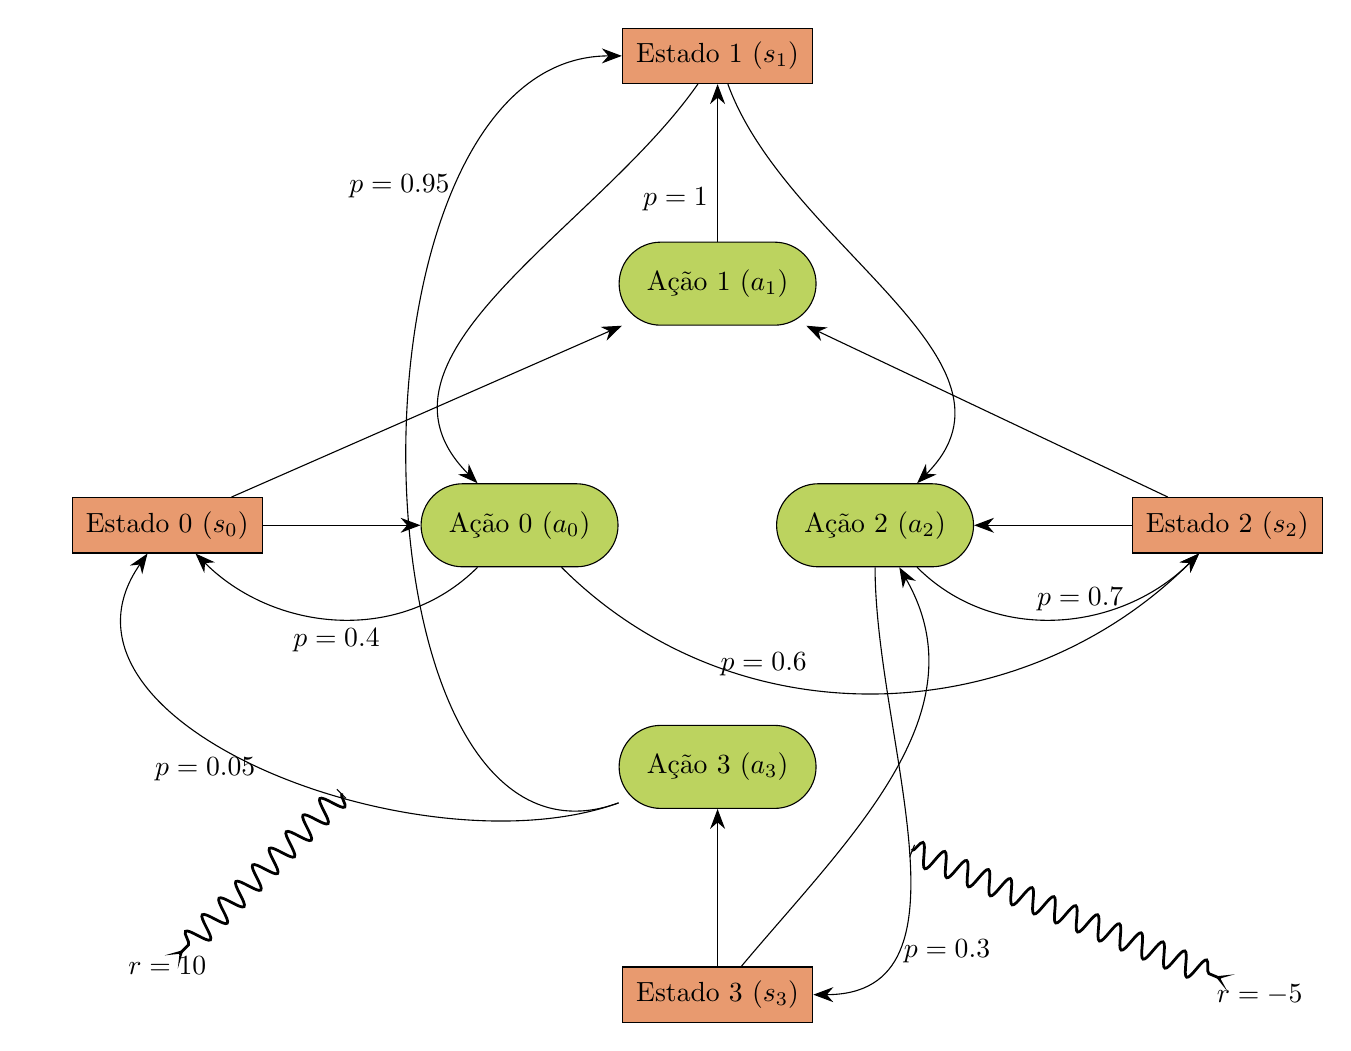
\begin{tikzpicture}
		\usetikzlibrary{arrows,automata,positioning,arrows.meta};
		\definecolor{statecolor}{HTML}{e89a6f};
		\definecolor{actioncolor}{HTML}{bcd35f};
		\tikzset{
			state/.style={
				shape=rectangle,
				draw=black,
				fill=statecolor,
				align=center,
				minimum height=2em,
				minimum width=4em,
				inner sep=5pt,
			},
			action/.style={
				shape=rectangle,
				draw=black,
				fill=actioncolor,
				align=center,
				inner sep=10pt,
				rounded corners=15pt,
			},
			reward/.style={
				|-,
				decoration={snake, amplitude=1.5mm, segment length=3mm},
				decorate,
				postaction={draw, line width=1pt, -{Stealth[scale=-0.8]}}
			},
			transition/.style={
				->,
				>={Stealth[scale=1.5]},
			}
		};
		\tikzset{node distance=2cm and 2cm}
    	\node[state] (s0) {Estado 0 ($s_0$)};

		\node[action, right=2cm of s0] (a0) {Ação 0 ($a_0$)};
		\node[action, above right=2cm and 0cm of a0] (a1) {Ação 1 ($a_1$)};
		\node[action, right=2cm of a0] (a2) {Ação 2 ($a_2$)};
		\node[action, below right=2cm and 0cm of a0] (a3) {Ação 3 ($a_3$)};

		\node[state, above=2cm of a1] (s1) {Estado 1 ($s_1$)};
		\node[state, right=2cm of a2] (s2) {Estado 2 ($s_2$)};
		\node[state, below=2cm of a3] (s3) {Estado 3 ($s_3$)};
		
		\node[draw=none, below right=2.8cm and 1cm of s0] (r0s) {};
		\node[draw=none, below=5cm of s0] (r0e) {$r=10$};
		
		\node[draw=none, above right=1.4cm and 1cm of s3] (r1s) {};
		\node[draw=none, right=5cm of s3] (r1e) {$r=-5$};
		
		\begin{scope} % actions
			\draw[transition] 
			(s0) 
			to
			(a0);
	
			\draw[transition] 
			(s0) 
			to
			(a1);
	
			\draw[transition] 
			(s1) 
			to[in=45, out=290]
			(a2);
	
			\draw[transition] 
			(s1) 
			to[in=135, out=235]
			(a0);
	
			\draw[transition] 
			(s2) 
			to
			(a1);
	
			\draw[transition] 
			(s2) 
			to
			(a2);
	
			\draw[transition] 
			(s3) 
			to
			(a3);
	
			\draw[transition] 
			(s3) 
			to[in=300, out=50]
			(a2);		
		\end{scope}
		
		\begin{scope} % transitions
			\draw[transition] 
			(a0)
			to[in=315, out=225] node[midway, below] 
			{$p = 0.4$} 
			(s0);
			
			\draw[transition] 
			(a0) 
			to[in=225, out=315] node[near start, right] 
			{$p = 0.6$} 
			(s2);
			
			\draw[transition] 
			(a1) 
			to[in=270, out=90] node[near start, left] 
			{$p = 1$} 
			(s1);
			
			\draw[transition] 
			(a2) 
			to[in=225, out=315] node[near end, left] 
			{$p = 0.7$} 
			(s2);
			
			\draw[transition] 
			(a2) 
			to[in=0, out=270] node[near end, right] 
			{$p = 0.3$} 
			(s3);
			
			\draw[transition] 
			(a3) 
			to[in=235, out=200] node[midway, left] 
			{$p = 0.05$} 
			(s0);
			
			\draw[transition] 
			(a3) 
			to[in=180, out=200] node[near end, left] 
			{$p = 0.95$} 
			(s1);
		\end{scope}
		
		\begin{scope}
			\draw[reward]
			(r0s)
			to
			(r0e);
			
			\draw[reward]
			(r1s)
			to
			(r1e);
			
		\end{scope}
	\end{tikzpicture}
\end{document}

	\caption{Discrete Markov Decision Process with 4 possible states and actions}
	\label{fig:mdp}
\end{figure}

\subsection{State Transition Distribution and Environment Evolution Dynamics}

The previously mentioned transition probability function $P$ is given in continuous time by the Kolmogorov forward equation for Markov Decission Processes:

\begin{equation}
	\frac{\partial P}{\partial t} \int_{\mathcal{S}} \mathcal{L}(s, a) P(s', t | s, a),
\end{equation}

Where $\mathcal{L}$ is the generator operator and governs the dynamics of the state transitions given the current time, and its expression is given by:

\begin{equation}
	\mathcal{L} f(s)=\int_{\mathcal{S}}(R(s, a, s')) Q\left(s, a, s^{\prime}\right) d s^{\prime}
\end{equation}

for all $s, s' \in \mathcal{S}$ and all times $t$ before market end $T$, that is, $t \le T$. 

In continuous-time and continuous-state MDPs, the state $S$ evolves as a continuous-time stochastic process, modern approaches to Reinforcement Learning require solving either numerically or approximating its transition probabilities. To do this, let us suppose $S$ represents the state of the system at time any given time $t$ after market start and before  or immediately at market end, such that $0 < t \leq T$, and we assume the evolution of the system follows a continuous-time Markov process with continuous state space and is known (In section <seção que vai explicar aqui> this strict supposition is removed and a model-free approach is used instead).

The key feature of a continuous-time Markov process is that the state transitions depend only on the current state and time, satisfying the Markov property, therefore the transition probabilities over an infinitesimally small time interval $\Delta t$ are governed by a transition rate function $\mathcal{L}(s, a)$. This function determines the rate at which the process transitions from the current state \( S_t = s \) to any neighboring state \( S_{t+\Delta t} = s' \) when the agent takes action $a$. In general, the transition rate is a function of the current state and the action chosen by the agent.

For a continuous-time Markov decision process, the state transition dynamics can't be represented by a time interval, and the Kolmogorov forward equation, which expresses the evolution of the probability distribution for the states over time is used. It is given by the following equation:

$$
\frac{d}{dt} P(s', t | s, a) = \int_{\mathcal{S}} \mathcal{L}(s' a, t) P(x| s, a, t) dx
$$

where $P(x, t | s, a)$ is the probability of being in state $x$ at time $t$, given previous state $s$, and $\mathcal{L}(s', a)$ is the transition rate from state $s'$ when action $a$ is taken.

The probability of transitioning from state \( X_t = X \) to a nearby state \( X' \) in an infinitesimal time \( \Delta t \) can be written as:

$$
\mathbb{P}(X_{t+\Delta t} = X' | X_t = X) \approx \Delta t \, Q(X, a), \quad X' \neq X,
$$
where \( Q(X, a) \) is the rate of transition from state \( X \) to state \( X' \).

For small time steps \( \Delta t \), the transition probability is approximately linear in \( \Delta t \), and the process remains in state \( X \) with probability \( 1 - \Delta t \, Q(X, a) \). Thus, the transition matrix can be written as:

$$
P(X, t + \Delta t | X, t) = 1 - \Delta t \, Q(X, a),
$$
$$
P(X', t + \Delta t | X, t) = \Delta t \, Q(X, a) \quad \text{for} \quad X' \neq X.
$$

The reward function in the continuous-time MDP is also typically time-dependent and reflects the instantaneous reward the agent receives when in state \( X \) and taking action \( a \). The reward function \( R(X, a) \) is defined as:

$$
R(X_t, a_t) = \text{Reward for taking action } a_t \text{ at state } X_t.
$$

The total accumulated reward over time is the integral of this instantaneous reward function.

To express the Bellman equation for continuous-time MDPs, we consider the value function \( V(X) \), which represents the expected total reward from state \( X \) under the optimal policy \( \pi^* \). The Bellman equation for a continuous-time MDP is:

$$
\frac{d}{dt} V(X) = \max_{a \in \mathcal{A}} \left[ R(X, a) + \sum_{X' \neq X} Q(X, a) \left( V(X') - V(X) \right) \right],
$$

where:
- \( R(X, a) \) is the reward obtained by taking action \( a \) at state \( X \),
- \( Q(X, a) \) is the transition rate function,
- \( V(X') \) is the value function for state \( X' \), and
- The summation term represents the expected change in value due to transitions to neighboring states.

The transition distribution \( \mathbb{P}(X' | X, a) \) in continuous time can be described as follows:

$$
\mathbb{P}(X' | X, a) = Q(X, a) \, \Delta t \quad \text{for} \quad X' \neq X,
$$

where \( \Delta t \) is a small time step, and \( Q(X, a) \) is the transition rate between states \( X \) and \( X' \) given action \( a \). This rate function governs the likelihood of moving from one state to another in the infinitesimal time step \( \Delta t \).

In summary, in continuous-time MDPs with continuous state spaces, the transition dynamics are characterized by the transition rate function \( Q(X, a) \), which determines the rates at which the state evolves based on the agent’s actions. The Bellman equation describes the evolution of the value function over time, and the reward function reflects the instantaneous reward the agent receives. The goal is to find the optimal policy that maximizes the expected cumulative reward.

This framework now describes the transition dynamics and how to mathematically formalize the continuous-time, continuous-state Markov decision process.

The RL environment is modeled as a MDP, consisting of the state space \( \mathcal{S} \), action space \( \mathcal{A} \), reward function \( r \), and some transition dynamics, either known or unknown. 

For testing our framework of inserting restrictions for the Market Maker trader, our market simulation is modeled as follows:

\begin{itemize}
	\item \textbf{State Space:} Let \( \mathbf{S}_t \) denote the state of the environment at time \( t \). The state includes the relative strength index (RSI), order imbalance (OI), micro price \( P_{\text{micro}} \), and the price level distances \( \Delta P_i \) at \( d \) levels of the LOB:
	
	$$
	\mathbf{S}_t = \left( \text{RSI}_t, \text{OI}_t, P_{\text{micro},t}, \Delta P_{1,t}, \Delta P_{2,t}, \dots, \Delta P_{d,t} \right) \in \mathbb{R}^3 \times \mathbb{R}^{2d}.
	$$
	
	The components of the state space are defined as follows:
	
	- \textbf{Order Imbalance (OI):} Order imbalance measures the relative difference between buy and sell orders at a given time. It is defined as:
	$$
	\text{OI}_t = \frac{Q_t^{\text{bid}} - Q_t^{\text{ask}}}{Q_t^{\text{bid}} + Q_t^{\text{ask}}},
	$$
	where \( Q_t^{\text{bid}} \) and \( Q_t^{\text{ask}} \) represent the total bid and ask quantities at time \( t \), respectively. \( \text{OI}_t \in [-1, 1] \), with \( \text{OI}_t = 1 \) indicating complete dominance of bid orders, and \( \text{OI}_t = -1 \) indicating ask order dominance.
	
	- \textbf{Relative Strength Index (RSI):} The RSI is a momentum indicator that compares the magnitude of recent gains to recent losses to evaluate overbought or oversold conditions. It is given by:
	$$
	\text{RSI}_t = 100 - \frac{100}{1 + \frac{\text{Average Gain}}{\text{Average Loss}}},
	$$
	where the \textit{Average Gain} and \textit{Average Loss} are computed over a rolling window (commonly 14 periods). Gains are the price increases during that window, while losses are the price decreases.
	
	- \textbf{Micro Price (\( P_{\text{micro}} \)):} The micro price is a weighted average of the best bid and ask prices, weighted by their respective quantities:
	$$
	P_{\text{micro},t} = \frac{P_t^{\text{ask}} Q_t^{\text{bid}} + P_t^{\text{bid}} Q_t^{\text{ask}}}{Q_t^{\text{bid}} + Q_t^{\text{ask}}},
	$$
	where \( P_t^{\text{ask}} \) and \( P_t^{\text{bid}} \) represent the best ask and bid prices at time \( t \).
	
	\item \textbf{Action Space:} The action space \( \mathcal{A}_t \) represents the decisions made by the agent at time \( t \), including the bid and ask spreads \( \delta_t^{\text{ask}}, \delta_t^{\text{bid}} \) and the corresponding order quantities \( q_t^{\text{ask}}, q_t^{\text{bid}} \). Formally:
	$$
	\mathbf{A}_t = \left( \delta_t^{\text{ask}}, \delta_t^{\text{bid}}, q_t^{\text{ask}}, q_t^{\text{bid}} \right) \in \mathbb{R}^2 \times \mathbb{Z}^2.
	$$
	
	\item \textbf{Reward Function:} The reward function \( r_t \in \mathbb{R} \) reflects the agent's profit and inventory risk. It is based on the spread and executed quantities, as well as the inventory cost.
\end{itemize}

The agent interacts with the environment by choosing actions \( \mathbf{A}_t \) in response to observed states \( \mathbf{S}_t \), and the goal is to maximize cumulative rewards over time. The system's evolution follows a , and the transition probabilities between states depend on the agent's actions.

\subsection{Chosen State and Action Space}
The limit order book is modeled as a continuous-time Markov chain, where the timing of events follows a \textit{Hawkes process} to capture the clustering of order arrivals.

The Hawkes process is a \textit{self-exciting process}, where the intensity \( \lambda(t) \) depends on past events. Formally, the intensity \( \lambda(t) \) evolves as:
$$
\lambda(t) = \mu + \sum_{t_i < t} \phi(t - t_i),
$$
where \( \mu > 0 \) is the baseline intensity, and \( \phi(t - t_i) \) is the \textit{kernel function} that governs the decay of influence from past events \( t_i \). A common choice for \( \phi \) is an exponential decay:
$$
\phi(t - t_i) = \alpha e^{-\beta (t - t_i)},
$$
where \( \alpha \) controls the magnitude of the self-excitation and \( \beta \) controls the rate of decay.

The bid and ask prices are modeled by \textit{Ornstein-Uhlenbeck (OU) processes} to capture the mean-reversion behavior of spreads:
$$
ds_t = \theta(\mu - s_t) dt + \sigma dW_t,
$$
where \( s_t \) is the market spread at time \( t \), \( \theta \) is the rate of mean reversion, \( \mu_{spread} \) is the long-term spread mean and \( \sigma \) its volatility. The Wiener process \( W_t \) is used to represent random market fluctuations.

The bid and ask spreads \( \delta_t^{\text{bid}} \) and \( \delta_t^{\text{ask}} \) for orders conditioned on their arrival follow normal distributions:
$$
\delta_t^{\text{ask}} \sim \mathcal{N}(\mu + M_{t-1} + s_t, \sigma^2), \quad a_t^{\text{bid}} \sim \mathcal{N}(\mu + M_{t-1} - s_t, \sigma^2),
$$
where \( \mu_{\text{ask}} \) and \( \mu_{\text{bid}} \) are the respective means and \( \Delta a_t \) is the spread adjustment.

Whenever a new limit order that narrows the bid-ask spread or a market order arrive the mid-price is updated to reflect the top-of-book orders. The mid-price \( M \) at time $t+1$ is then obtained by averaging the maximum and minimum bid and ask prices in the book:

$$
M_{t+1} = \frac{2M_t + \delta^{ask}_{t} - \delta^{bid}_{t}}{2} 
\sim \mathcal{N}(\mu + M_{t}, \frac{\sigma^2}{2})
$$

The average of the best bid and ask prices therefore evolves according to a \textit{Brownian Motion} process:
$$
dM_t = \mu dt + \frac{\sigma^2}{2} dW_t,
$$
where \( W_t \) is a Wiener process.

The order quantities \( q_t^{\text{ask}} \) and \( q_t^{\text{bid}} \) are modeled as Poisson random variables:
$$
q_t^{\text{ask}}, q_t^{\text{bid}} \sim \text{Poisson}(\lambda_q),
$$
where \( \lambda_q \) is the average order size.

\subsection{Decision Process and Agent Objective}
The agent’s goal is to maximize its utility, which for our model is based on a Profit and Loss (PnL) score while still managing inventory risk. The choosen reward function is based on a risk-aversion enforced utility function, specifically the \textit{constant absolute risk aversion (CARA)}:
$$
R_t = U(\text{PnL}_t) = -e^{-\gamma \cdot \text{PnL}_t},
$$
where \( \gamma \) is the risk aversion parameter.

The PnL at time \( t \) is computed as:
$$
\text{PnL}_t = \delta_t^{\text{ask}} q_t^{\text{ask}} - \delta_t^{\text{bid}} q_t^{\text{bid}} + \text{I}_t \cdot \Delta M_t.
$$

The agent starting penalty for holding large inventory positions  is discounted from the \textit{PnL} score, as follows:
$$
\text{Penalty}_t = \eta \left( \text{Inventory}_t \cdot \Delta M_t \right)^+,
$$
$$
\text{PnL}_t := \text{PnL}_t - \text{Penalty}_t
$$
where \( \eta \) is the penalty factor applied to positive inventory changes.

The overall objective is to maximize cumulative utility while minimizing risk associated with inventory positions, and later insert restrictions so the risk for inventory is either limited at zero at market close, or incurring in larger penalties on the received rewards.